\documentclass[twoside]{book}

% Packages required by doxygen
\usepackage{fixltx2e}
\usepackage{calc}
\usepackage{doxygen}
\usepackage[export]{adjustbox} % also loads graphicx
\usepackage{graphicx}
\usepackage[utf8]{inputenc}
\usepackage{makeidx}
\usepackage{multicol}
\usepackage{multirow}
\PassOptionsToPackage{warn}{textcomp}
\usepackage{textcomp}
\usepackage[nointegrals]{wasysym}
\usepackage[table]{xcolor}

% Font selection
\usepackage[T1]{fontenc}
\usepackage[scaled=.90]{helvet}
\usepackage{courier}
\usepackage{amssymb}
\usepackage{sectsty}
\renewcommand{\familydefault}{\sfdefault}
\allsectionsfont{%
  \fontseries{bc}\selectfont%
  \color{darkgray}%
}
\renewcommand{\DoxyLabelFont}{%
  \fontseries{bc}\selectfont%
  \color{darkgray}%
}
\newcommand{\+}{\discretionary{\mbox{\scriptsize$\hookleftarrow$}}{}{}}

% Page & text layout
\usepackage{geometry}
\geometry{%
  a4paper,%
  top=2.5cm,%
  bottom=2.5cm,%
  left=2.5cm,%
  right=2.5cm%
}
\tolerance=750
\hfuzz=15pt
\hbadness=750
\setlength{\emergencystretch}{15pt}
\setlength{\parindent}{0cm}
\setlength{\parskip}{3ex plus 2ex minus 2ex}
\makeatletter
\renewcommand{\paragraph}{%
  \@startsection{paragraph}{4}{0ex}{-1.0ex}{1.0ex}{%
    \normalfont\normalsize\bfseries\SS@parafont%
  }%
}
\renewcommand{\subparagraph}{%
  \@startsection{subparagraph}{5}{0ex}{-1.0ex}{1.0ex}{%
    \normalfont\normalsize\bfseries\SS@subparafont%
  }%
}
\makeatother

% Headers & footers
\usepackage{fancyhdr}
\pagestyle{fancyplain}
\fancyhead[LE]{\fancyplain{}{\bfseries\thepage}}
\fancyhead[CE]{\fancyplain{}{}}
\fancyhead[RE]{\fancyplain{}{\bfseries\leftmark}}
\fancyhead[LO]{\fancyplain{}{\bfseries\rightmark}}
\fancyhead[CO]{\fancyplain{}{}}
\fancyhead[RO]{\fancyplain{}{\bfseries\thepage}}
\fancyfoot[LE]{\fancyplain{}{}}
\fancyfoot[CE]{\fancyplain{}{}}
\fancyfoot[RE]{\fancyplain{}{\bfseries\scriptsize Generated by Doxygen }}
\fancyfoot[LO]{\fancyplain{}{\bfseries\scriptsize Generated by Doxygen }}
\fancyfoot[CO]{\fancyplain{}{}}
\fancyfoot[RO]{\fancyplain{}{}}
\renewcommand{\footrulewidth}{0.4pt}
\renewcommand{\chaptermark}[1]{%
  \markboth{#1}{}%
}
\renewcommand{\sectionmark}[1]{%
  \markright{\thesection\ #1}%
}

% Indices & bibliography
\usepackage{natbib}
\usepackage[titles]{tocloft}
\setcounter{tocdepth}{3}
\setcounter{secnumdepth}{5}
\makeindex

% Custom commands
\newcommand{\clearemptydoublepage}{%
  \newpage{\pagestyle{empty}\cleardoublepage}%
}

\usepackage{caption}
\captionsetup{labelsep=space,justification=centering,font={bf},singlelinecheck=off,skip=4pt,position=top}

%===== C O N T E N T S =====

\begin{document}

% Titlepage & ToC
\pagenumbering{alph}
\begin{titlepage}
\vspace*{7cm}
\begin{center}%
{\Large Life }\\
\vspace*{1cm}
{\large Generated by Doxygen 1.8.13}\\
\end{center}
\end{titlepage}
\clearemptydoublepage
\pagenumbering{roman}
\tableofcontents
\clearemptydoublepage
\pagenumbering{arabic}

%--- Begin generated contents ---
\chapter{Hierarchical Index}
\section{Class Hierarchy}
This inheritance list is sorted roughly, but not completely, alphabetically\+:\begin{DoxyCompactList}
\item \contentsline{section}{Cell}{\pageref{classCell}}{}
\item \contentsline{section}{Grid}{\pageref{classGrid}}{}
\item \contentsline{section}{Organism}{\pageref{classOrganism}}{}
\begin{DoxyCompactList}
\item \contentsline{section}{Ant}{\pageref{classAnt}}{}
\item \contentsline{section}{Doodlebug}{\pageref{classDoodlebug}}{}
\end{DoxyCompactList}
\item \contentsline{section}{Production}{\pageref{classProduction}}{}
\item \contentsline{section}{Tests2}{\pageref{classTests2}}{}
\end{DoxyCompactList}

\chapter{Data Structure Index}
\section{Data Structures}
Here are the data structures with brief descriptions\+:\begin{DoxyCompactList}
\item\contentsline{section}{\textbf{ Ant} }{\pageref{classAnt}}{}
\item\contentsline{section}{\textbf{ Cell} }{\pageref{classCell}}{}
\item\contentsline{section}{\textbf{ Doodlebug} }{\pageref{classDoodlebug}}{}
\item\contentsline{section}{\textbf{ Grid} }{\pageref{classGrid}}{}
\item\contentsline{section}{\textbf{ Organism} }{\pageref{classOrganism}}{}
\item\contentsline{section}{\textbf{ Production} }{\pageref{classProduction}}{}
\item\contentsline{section}{\textbf{ Tests2} }{\pageref{classTests2}}{}
\end{DoxyCompactList}

\chapter{File Index}
\section{File List}
Here is a list of all files with brief descriptions\+:\begin{DoxyCompactList}
\item\contentsline{section}{\textbf{ Ant.\+cpp} }{\pageref{Ant_8cpp}}{}
\item\contentsline{section}{\textbf{ Ant.\+h} }{\pageref{Ant_8h}}{}
\item\contentsline{section}{\textbf{ Ants\+And\+Doodles.\+cpp} }{\pageref{AntsAndDoodles_8cpp}}{}
\item\contentsline{section}{\textbf{ Cell.\+cpp} }{\pageref{Cell_8cpp}}{}
\item\contentsline{section}{\textbf{ Cell.\+h} }{\pageref{Cell_8h}}{}
\item\contentsline{section}{\textbf{ Doodlebug.\+cpp} }{\pageref{Doodlebug_8cpp}}{}
\item\contentsline{section}{\textbf{ Doodlebug.\+h} }{\pageref{Doodlebug_8h}}{}
\item\contentsline{section}{\textbf{ Grid.\+cpp} }{\pageref{Grid_8cpp}}{}
\item\contentsline{section}{\textbf{ Grid.\+h} }{\pageref{Grid_8h}}{}
\item\contentsline{section}{\textbf{ Organism.\+cpp} }{\pageref{Organism_8cpp}}{}
\item\contentsline{section}{\textbf{ Organism.\+h} }{\pageref{Organism_8h}}{}
\item\contentsline{section}{\textbf{ Production.\+cpp} }{\pageref{Production_8cpp}}{}
\item\contentsline{section}{\textbf{ Production.\+h} }{\pageref{Production_8h}}{}
\item\contentsline{section}{\textbf{ Tests2.\+cpp} }{\pageref{Tests2_8cpp}}{}
\item\contentsline{section}{\textbf{ Tests2.\+h} }{\pageref{Tests2_8h}}{}
\end{DoxyCompactList}

\chapter{Data Structure Documentation}
\section{Ant Class Reference}
\label{classAnt}\index{Ant@{Ant}}


{\ttfamily \#include $<$Ant.\+h$>$}

Inheritance diagram for Ant\+:\begin{figure}[H]
\begin{center}
\leavevmode
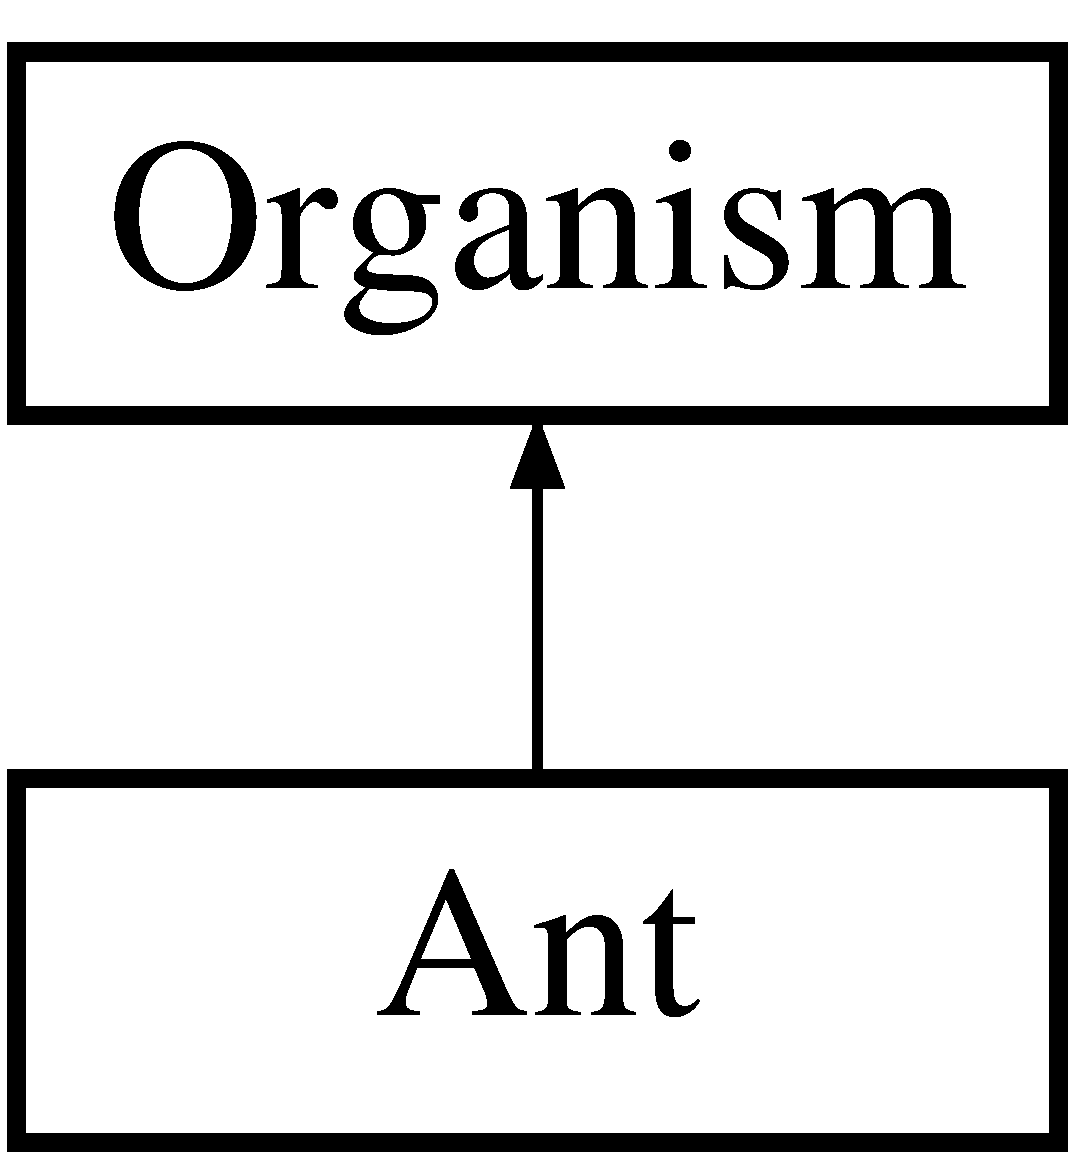
\includegraphics[height=2.000000cm]{classAnt}
\end{center}
\end{figure}
\subsection*{Public Member Functions}
\begin{DoxyCompactItemize}
\item 
\textbf{ Ant} ()
\item 
\textbf{ Ant} (int r=0, int c=0)
\item 
int \textbf{ get\+Row} ()
\item 
int \textbf{ get\+Col} ()
\item 
int \textbf{ get\+Breed\+Counter} ()
\item 
int \textbf{ move} (\textbf{ Grid} $\ast$grid)
\item 
void \textbf{ move\+Helper} (\textbf{ Grid} $\ast$grid, int dir)
\item 
void \textbf{ breed\+Helper} (\textbf{ Grid} $\ast$grid, int dir)
\item 
bool \textbf{ breed} (\textbf{ Grid} $\ast$grid)
\item 
\textbf{ $\sim$\+Ant} ()
\end{DoxyCompactItemize}
\subsection*{Private Attributes}
\begin{DoxyCompactItemize}
\item 
int \textbf{ row} = 0
\item 
int \textbf{ col} = 0
\item 
int \textbf{ breed\+Counter} =0
\end{DoxyCompactItemize}


\subsection{Constructor \& Destructor Documentation}
\mbox{\label{classAnt_ad6c1a8f70419877f7a3e2c9c557f913d}} 
\index{Ant@{Ant}!Ant@{Ant}}
\index{Ant@{Ant}!Ant@{Ant}}
\subsubsection{Ant()\hspace{0.1cm}{\footnotesize\ttfamily [1/2]}}
{\footnotesize\ttfamily Ant\+::\+Ant (\begin{DoxyParamCaption}{ }\end{DoxyParamCaption})}

\mbox{\label{classAnt_afcb9b285a5aa4b329e7eb5783970d85f}} 
\index{Ant@{Ant}!Ant@{Ant}}
\index{Ant@{Ant}!Ant@{Ant}}
\subsubsection{Ant()\hspace{0.1cm}{\footnotesize\ttfamily [2/2]}}
{\footnotesize\ttfamily Ant\+::\+Ant (\begin{DoxyParamCaption}\item[{int}]{r = {\ttfamily 0},  }\item[{int}]{c = {\ttfamily 0} }\end{DoxyParamCaption})}



References col, and row.

\mbox{\label{classAnt_a33ca6bd592236726a18a2159908e4116}} 
\index{Ant@{Ant}!````~Ant@{$\sim$\+Ant}}
\index{````~Ant@{$\sim$\+Ant}!Ant@{Ant}}
\subsubsection{$\sim$\+Ant()}
{\footnotesize\ttfamily Ant\+::$\sim$\+Ant (\begin{DoxyParamCaption}{ }\end{DoxyParamCaption})}



\subsection{Member Function Documentation}
\mbox{\label{classAnt_af899faded61186f5ca27e43cee1463ba}} 
\index{Ant@{Ant}!breed@{breed}}
\index{breed@{breed}!Ant@{Ant}}
\subsubsection{breed()}
{\footnotesize\ttfamily bool Ant\+::breed (\begin{DoxyParamCaption}\item[{\textbf{ Grid} $\ast$}]{grid }\end{DoxyParamCaption})\hspace{0.3cm}{\ttfamily [virtual]}}



Implements \textbf{ Organism} \doxyref{}{p.}{classOrganism_a423246fb1dee94db6c8c3b08fba57ead}.



References breed\+Counter, breed\+Helper(), col, empty, Grid\+::find\+Neighbours(), Grid\+::rand\+Int(), and row.



Referenced by move().

\mbox{\label{classAnt_aa302446f5fe2068ad34fdb1d66fd7ede}} 
\index{Ant@{Ant}!breed\+Helper@{breed\+Helper}}
\index{breed\+Helper@{breed\+Helper}!Ant@{Ant}}
\subsubsection{breed\+Helper()}
{\footnotesize\ttfamily void Ant\+::breed\+Helper (\begin{DoxyParamCaption}\item[{\textbf{ Grid} $\ast$}]{grid,  }\item[{int}]{dir }\end{DoxyParamCaption})}



References ant, col, Grid\+::get\+Board(), Cell\+::\+New\+Ptr(), row, and Grid\+::set\+Cell\+Occupant().



Referenced by breed().

\mbox{\label{classAnt_abc55a1896436ad4907fa1f9520657e6d}} 
\index{Ant@{Ant}!get\+Breed\+Counter@{get\+Breed\+Counter}}
\index{get\+Breed\+Counter@{get\+Breed\+Counter}!Ant@{Ant}}
\subsubsection{get\+Breed\+Counter()}
{\footnotesize\ttfamily int Ant\+::get\+Breed\+Counter (\begin{DoxyParamCaption}{ }\end{DoxyParamCaption})}



References breed\+Counter.

\mbox{\label{classAnt_a3c31dc577ebf913d246c16db3b1ed8e2}} 
\index{Ant@{Ant}!get\+Col@{get\+Col}}
\index{get\+Col@{get\+Col}!Ant@{Ant}}
\subsubsection{get\+Col()}
{\footnotesize\ttfamily int Ant\+::get\+Col (\begin{DoxyParamCaption}{ }\end{DoxyParamCaption})}



References col.

\mbox{\label{classAnt_acef79a2f69e2493dc3067db4b41783a9}} 
\index{Ant@{Ant}!get\+Row@{get\+Row}}
\index{get\+Row@{get\+Row}!Ant@{Ant}}
\subsubsection{get\+Row()}
{\footnotesize\ttfamily int Ant\+::get\+Row (\begin{DoxyParamCaption}{ }\end{DoxyParamCaption})}



References row.

\mbox{\label{classAnt_a6806cb12fd6e7eea2ff74ea8aa33ce28}} 
\index{Ant@{Ant}!move@{move}}
\index{move@{move}!Ant@{Ant}}
\subsubsection{move()}
{\footnotesize\ttfamily int Ant\+::move (\begin{DoxyParamCaption}\item[{\textbf{ Grid} $\ast$}]{grid }\end{DoxyParamCaption})\hspace{0.3cm}{\ttfamily [virtual]}}



Implements \textbf{ Organism} \doxyref{}{p.}{classOrganism_a2627a1917b919ab131d40d868b966020}.



References breed(), breed\+Counter, col, empty, Grid\+::find\+Neighbours(), Grid\+::get\+Board(), move\+Helper(), Grid\+::rand\+Int(), row, Grid\+::set\+Cell\+Occupant(), and Cell\+::set\+Ptr().

\mbox{\label{classAnt_a3fccb8a3cd08fea185e242272674443b}} 
\index{Ant@{Ant}!move\+Helper@{move\+Helper}}
\index{move\+Helper@{move\+Helper}!Ant@{Ant}}
\subsubsection{move\+Helper()}
{\footnotesize\ttfamily void Ant\+::move\+Helper (\begin{DoxyParamCaption}\item[{\textbf{ Grid} $\ast$}]{grid,  }\item[{int}]{dir }\end{DoxyParamCaption})}



References ant, col, Grid\+::get\+Board(), Cell\+::get\+Ptr(), row, Grid\+::set\+Cell\+Occupant(), and Cell\+::set\+Ptr().



Referenced by move().



\subsection{Field Documentation}
\mbox{\label{classAnt_a0a7fef71b2bcfb5bc3df0d588745dc01}} 
\index{Ant@{Ant}!breed\+Counter@{breed\+Counter}}
\index{breed\+Counter@{breed\+Counter}!Ant@{Ant}}
\subsubsection{breed\+Counter}
{\footnotesize\ttfamily int Ant\+::breed\+Counter =0\hspace{0.3cm}{\ttfamily [private]}}



Referenced by breed(), get\+Breed\+Counter(), and move().

\mbox{\label{classAnt_afe21bedec87ea26e3db74857960a78c6}} 
\index{Ant@{Ant}!col@{col}}
\index{col@{col}!Ant@{Ant}}
\subsubsection{col}
{\footnotesize\ttfamily int Ant\+::col = 0\hspace{0.3cm}{\ttfamily [private]}}



Referenced by Ant(), breed(), breed\+Helper(), get\+Col(), move(), and move\+Helper().

\mbox{\label{classAnt_abf712c4a02e999938c7d79557a8fc24b}} 
\index{Ant@{Ant}!row@{row}}
\index{row@{row}!Ant@{Ant}}
\subsubsection{row}
{\footnotesize\ttfamily int Ant\+::row = 0\hspace{0.3cm}{\ttfamily [private]}}



Referenced by Ant(), breed(), breed\+Helper(), get\+Row(), move(), and move\+Helper().



The documentation for this class was generated from the following files\+:\begin{DoxyCompactItemize}
\item 
\textbf{ Ant.\+h}\item 
\textbf{ Ant.\+cpp}\end{DoxyCompactItemize}

\section{Cell Class Reference}
\label{classCell}\index{Cell@{Cell}}


{\ttfamily \#include $<$Cell.\+h$>$}

\subsection*{Public Member Functions}
\begin{DoxyCompactItemize}
\item 
\textbf{ Cell} ()
\item 
bool \textbf{ set\+Occupant} (\textbf{ occupation\+Status} g)
\item 
void \textbf{ New\+Ptr} (int r, int c, \textbf{ occupation\+Status} g)
\item 
\textbf{ Organism} $\ast$ \textbf{ get\+Ptr} ()
\item 
void \textbf{ set\+Ptr} (\textbf{ Organism} $\ast$new\+Ptr)
\item 
\textbf{ occupation\+Status} \textbf{ get\+Occupant} ()
\item 
virtual \textbf{ $\sim$\+Cell} ()
\end{DoxyCompactItemize}
\subsection*{Data Fields}
\begin{DoxyCompactItemize}
\item 
\textbf{ occupation\+Status} \textbf{ guest}
\item 
\textbf{ Organism} $\ast$ \textbf{ ptr}
\end{DoxyCompactItemize}


\subsection{Constructor \& Destructor Documentation}
\mbox{\label{classCell_a394510643e8664cf12b5efaf5cb99f71}} 
\index{Cell@{Cell}!Cell@{Cell}}
\index{Cell@{Cell}!Cell@{Cell}}
\subsubsection{Cell()}
{\footnotesize\ttfamily Cell\+::\+Cell (\begin{DoxyParamCaption}{ }\end{DoxyParamCaption})}



References empty, guest, and ptr.

\mbox{\label{classCell_a9fa559f7a28e2b4336c6879ca09304d8}} 
\index{Cell@{Cell}!````~Cell@{$\sim$\+Cell}}
\index{````~Cell@{$\sim$\+Cell}!Cell@{Cell}}
\subsubsection{$\sim$\+Cell()}
{\footnotesize\ttfamily Cell\+::$\sim$\+Cell (\begin{DoxyParamCaption}{ }\end{DoxyParamCaption})\hspace{0.3cm}{\ttfamily [virtual]}}



Referenced by Grid\+::$\sim$\+Grid().



\subsection{Member Function Documentation}
\mbox{\label{classCell_a7dcb8bc75a2e2591b3fd52b5f7c28ab1}} 
\index{Cell@{Cell}!get\+Occupant@{get\+Occupant}}
\index{get\+Occupant@{get\+Occupant}!Cell@{Cell}}
\subsubsection{get\+Occupant()}
{\footnotesize\ttfamily \textbf{ occupation\+Status} Cell\+::get\+Occupant (\begin{DoxyParamCaption}{ }\end{DoxyParamCaption})}



References guest.



Referenced by Grid\+::get\+Cell\+Occupant().

\mbox{\label{classCell_a1009c9d271700e6ee9a7da1eca77802a}} 
\index{Cell@{Cell}!get\+Ptr@{get\+Ptr}}
\index{get\+Ptr@{get\+Ptr}!Cell@{Cell}}
\subsubsection{get\+Ptr()}
{\footnotesize\ttfamily \textbf{ Organism} $\ast$ Cell\+::get\+Ptr (\begin{DoxyParamCaption}{ }\end{DoxyParamCaption})}



References ptr.



Referenced by Tests2\+::ants\+Breed\+Test(), Tests2\+::ants\+Die\+Test(), Tests2\+::ants\+Move\+Test(), Tests2\+::doodle\+Breed\+Test(), Tests2\+::doodle\+Dietest(), Tests2\+::doodle\+Move\+Test(), Ant\+::move\+Helper(), Doodlebug\+::move\+Helper(), and Production\+::run\+Production().

\mbox{\label{classCell_a393e1ebaeb895c634c9402e7c16306e2}} 
\index{Cell@{Cell}!New\+Ptr@{New\+Ptr}}
\index{New\+Ptr@{New\+Ptr}!Cell@{Cell}}
\subsubsection{New\+Ptr()}
{\footnotesize\ttfamily void Cell\+::\+New\+Ptr (\begin{DoxyParamCaption}\item[{int}]{r,  }\item[{int}]{c,  }\item[{\textbf{ occupation\+Status}}]{g }\end{DoxyParamCaption})}



References ant, doodlebug, empty, and ptr.



Referenced by Tests2\+::ants\+Breed\+Test(), Tests2\+::ants\+Die\+Test(), Tests2\+::ants\+Move\+Test(), Ant\+::breed\+Helper(), Doodlebug\+::breed\+Helper(), Tests2\+::doodle\+Breed\+Test(), Tests2\+::doodle\+Dietest(), Tests2\+::doodle\+Move\+Test(), and Production\+::run\+Production().

\mbox{\label{classCell_a2346933316b45d87264d50e563c2f895}} 
\index{Cell@{Cell}!set\+Occupant@{set\+Occupant}}
\index{set\+Occupant@{set\+Occupant}!Cell@{Cell}}
\subsubsection{set\+Occupant()}
{\footnotesize\ttfamily bool Cell\+::set\+Occupant (\begin{DoxyParamCaption}\item[{\textbf{ occupation\+Status}}]{g }\end{DoxyParamCaption})}



References empty, and guest.



Referenced by Grid\+::set\+Cell\+Occupant().

\mbox{\label{classCell_a99ffc4814041c8b8482cabe20a25a17e}} 
\index{Cell@{Cell}!set\+Ptr@{set\+Ptr}}
\index{set\+Ptr@{set\+Ptr}!Cell@{Cell}}
\subsubsection{set\+Ptr()}
{\footnotesize\ttfamily void Cell\+::set\+Ptr (\begin{DoxyParamCaption}\item[{\textbf{ Organism} $\ast$}]{new\+Ptr }\end{DoxyParamCaption})}



References ptr.



Referenced by Doodlebug\+::eat(), Ant\+::move(), Doodlebug\+::move(), Ant\+::move\+Helper(), and Doodlebug\+::move\+Helper().



\subsection{Field Documentation}
\mbox{\label{classCell_aafc273a5125cf29742a8df6f5a5a881c}} 
\index{Cell@{Cell}!guest@{guest}}
\index{guest@{guest}!Cell@{Cell}}
\subsubsection{guest}
{\footnotesize\ttfamily \textbf{ occupation\+Status} Cell\+::guest}



Referenced by Cell(), get\+Occupant(), and set\+Occupant().

\mbox{\label{classCell_a0f787af5a8409c38ded198420fe8afae}} 
\index{Cell@{Cell}!ptr@{ptr}}
\index{ptr@{ptr}!Cell@{Cell}}
\subsubsection{ptr}
{\footnotesize\ttfamily \textbf{ Organism}$\ast$ Cell\+::ptr}



Referenced by Cell(), get\+Ptr(), New\+Ptr(), and set\+Ptr().



The documentation for this class was generated from the following files\+:\begin{DoxyCompactItemize}
\item 
\textbf{ Cell.\+h}\item 
\textbf{ Cell.\+cpp}\end{DoxyCompactItemize}

\section{Doodlebug Class Reference}
\label{classDoodlebug}\index{Doodlebug@{Doodlebug}}


{\ttfamily \#include $<$Doodlebug.\+h$>$}

Inheritance diagram for Doodlebug\+:\begin{figure}[H]
\begin{center}
\leavevmode
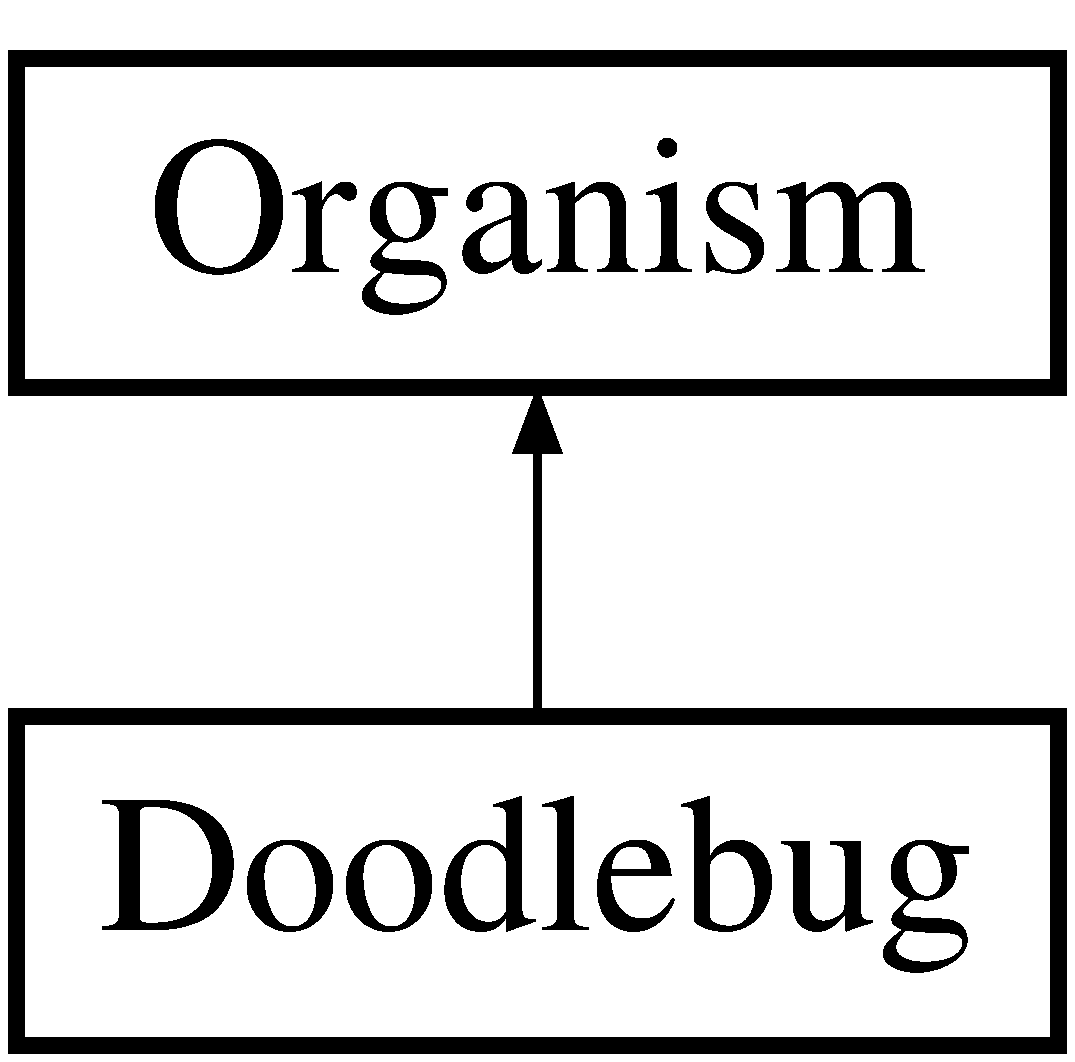
\includegraphics[height=2.000000cm]{classDoodlebug}
\end{center}
\end{figure}
\subsection*{Public Member Functions}
\begin{DoxyCompactItemize}
\item 
\textbf{ Doodlebug} ()
\item 
\textbf{ Doodlebug} (int r=0, int c=0)
\item 
int \textbf{ get\+Row} ()
\item 
int \textbf{ get\+Col} ()
\item 
int \textbf{ get\+Breed\+Counter} ()
\item 
int \textbf{ get\+Death\+Counter} ()
\item 
int \textbf{ move} (\textbf{ Grid} $\ast$grid)
\item 
void \textbf{ move\+Helper} (\textbf{ Grid} $\ast$grid, int dir)
\item 
void \textbf{ breed\+Helper} (\textbf{ Grid} $\ast$grid, int dir)
\item 
bool \textbf{ breed} (\textbf{ Grid} $\ast$grid)
\item 
int \textbf{ eat} (\textbf{ Grid} $\ast$grid, bool $\ast$arr\+Ants)
\item 
virtual \textbf{ $\sim$\+Doodlebug} ()
\end{DoxyCompactItemize}
\subsection*{Private Attributes}
\begin{DoxyCompactItemize}
\item 
int \textbf{ row} = 0
\item 
int \textbf{ col} = 0
\item 
int \textbf{ breed\+Counter} =0
\item 
int \textbf{ death\+Count} =0
\end{DoxyCompactItemize}


\subsection{Constructor \& Destructor Documentation}
\mbox{\label{classDoodlebug_afb2796ea39a6ffa13d4f54ac68dd52fc}} 
\index{Doodlebug@{Doodlebug}!Doodlebug@{Doodlebug}}
\index{Doodlebug@{Doodlebug}!Doodlebug@{Doodlebug}}
\subsubsection{Doodlebug()\hspace{0.1cm}{\footnotesize\ttfamily [1/2]}}
{\footnotesize\ttfamily Doodlebug\+::\+Doodlebug (\begin{DoxyParamCaption}{ }\end{DoxyParamCaption})}

\mbox{\label{classDoodlebug_a5c450345bdd9e9895f589b8321a850a3}} 
\index{Doodlebug@{Doodlebug}!Doodlebug@{Doodlebug}}
\index{Doodlebug@{Doodlebug}!Doodlebug@{Doodlebug}}
\subsubsection{Doodlebug()\hspace{0.1cm}{\footnotesize\ttfamily [2/2]}}
{\footnotesize\ttfamily Doodlebug\+::\+Doodlebug (\begin{DoxyParamCaption}\item[{int}]{r = {\ttfamily 0},  }\item[{int}]{c = {\ttfamily 0} }\end{DoxyParamCaption})}



References col, and row.

\mbox{\label{classDoodlebug_ac318cc9acbd9a3af52348a236070d891}} 
\index{Doodlebug@{Doodlebug}!````~Doodlebug@{$\sim$\+Doodlebug}}
\index{````~Doodlebug@{$\sim$\+Doodlebug}!Doodlebug@{Doodlebug}}
\subsubsection{$\sim$\+Doodlebug()}
{\footnotesize\ttfamily Doodlebug\+::$\sim$\+Doodlebug (\begin{DoxyParamCaption}{ }\end{DoxyParamCaption})\hspace{0.3cm}{\ttfamily [virtual]}}



\subsection{Member Function Documentation}
\mbox{\label{classDoodlebug_a6ab3919da6f9404f1f3af05f0bbde13c}} 
\index{Doodlebug@{Doodlebug}!breed@{breed}}
\index{breed@{breed}!Doodlebug@{Doodlebug}}
\subsubsection{breed()}
{\footnotesize\ttfamily bool Doodlebug\+::breed (\begin{DoxyParamCaption}\item[{\textbf{ Grid} $\ast$}]{grid }\end{DoxyParamCaption})\hspace{0.3cm}{\ttfamily [virtual]}}



Implements \textbf{ Organism} \doxyref{}{p.}{classOrganism_a423246fb1dee94db6c8c3b08fba57ead}.



References breed\+Counter, breed\+Helper(), col, empty, Grid\+::find\+Neighbours(), Grid\+::rand\+Int(), and row.



Referenced by move().

\mbox{\label{classDoodlebug_a0c00c2c7d106c8fc298e55be562238d2}} 
\index{Doodlebug@{Doodlebug}!breed\+Helper@{breed\+Helper}}
\index{breed\+Helper@{breed\+Helper}!Doodlebug@{Doodlebug}}
\subsubsection{breed\+Helper()}
{\footnotesize\ttfamily void Doodlebug\+::breed\+Helper (\begin{DoxyParamCaption}\item[{\textbf{ Grid} $\ast$}]{grid,  }\item[{int}]{dir }\end{DoxyParamCaption})}



References col, doodlebug, Grid\+::get\+Board(), Cell\+::\+New\+Ptr(), row, and Grid\+::set\+Cell\+Occupant().



Referenced by breed().

\mbox{\label{classDoodlebug_a2737e34be4b0d57a188eb35bb7666412}} 
\index{Doodlebug@{Doodlebug}!eat@{eat}}
\index{eat@{eat}!Doodlebug@{Doodlebug}}
\subsubsection{eat()}
{\footnotesize\ttfamily int Doodlebug\+::eat (\begin{DoxyParamCaption}\item[{\textbf{ Grid} $\ast$}]{grid,  }\item[{bool $\ast$}]{arr\+Ants }\end{DoxyParamCaption})}



References breed\+Counter, col, death\+Count, empty, Grid\+::get\+Board(), move\+Helper(), Grid\+::rand\+Int(), row, Grid\+::set\+Cell\+Occupant(), and Cell\+::set\+Ptr().



Referenced by move().

\mbox{\label{classDoodlebug_acf526002dc3072874ca207765b2124fb}} 
\index{Doodlebug@{Doodlebug}!get\+Breed\+Counter@{get\+Breed\+Counter}}
\index{get\+Breed\+Counter@{get\+Breed\+Counter}!Doodlebug@{Doodlebug}}
\subsubsection{get\+Breed\+Counter()}
{\footnotesize\ttfamily int Doodlebug\+::get\+Breed\+Counter (\begin{DoxyParamCaption}{ }\end{DoxyParamCaption})}



References breed\+Counter.

\mbox{\label{classDoodlebug_aa311d47bffaf0e68785b8a1472537807}} 
\index{Doodlebug@{Doodlebug}!get\+Col@{get\+Col}}
\index{get\+Col@{get\+Col}!Doodlebug@{Doodlebug}}
\subsubsection{get\+Col()}
{\footnotesize\ttfamily int Doodlebug\+::get\+Col (\begin{DoxyParamCaption}{ }\end{DoxyParamCaption})}



References death\+Count.

\mbox{\label{classDoodlebug_afa74bc4327951a7016394e1e4b699358}} 
\index{Doodlebug@{Doodlebug}!get\+Death\+Counter@{get\+Death\+Counter}}
\index{get\+Death\+Counter@{get\+Death\+Counter}!Doodlebug@{Doodlebug}}
\subsubsection{get\+Death\+Counter()}
{\footnotesize\ttfamily int Doodlebug\+::get\+Death\+Counter (\begin{DoxyParamCaption}{ }\end{DoxyParamCaption})}



References death\+Count.

\mbox{\label{classDoodlebug_afb3ba6dc552b2c83caf316405db616ec}} 
\index{Doodlebug@{Doodlebug}!get\+Row@{get\+Row}}
\index{get\+Row@{get\+Row}!Doodlebug@{Doodlebug}}
\subsubsection{get\+Row()}
{\footnotesize\ttfamily int Doodlebug\+::get\+Row (\begin{DoxyParamCaption}{ }\end{DoxyParamCaption})}



References row.

\mbox{\label{classDoodlebug_a5f28800e091fbeaabd57079b0c36e997}} 
\index{Doodlebug@{Doodlebug}!move@{move}}
\index{move@{move}!Doodlebug@{Doodlebug}}
\subsubsection{move()}
{\footnotesize\ttfamily int Doodlebug\+::move (\begin{DoxyParamCaption}\item[{\textbf{ Grid} $\ast$}]{grid }\end{DoxyParamCaption})\hspace{0.3cm}{\ttfamily [virtual]}}



Implements \textbf{ Organism} \doxyref{}{p.}{classOrganism_a2627a1917b919ab131d40d868b966020}.



References ant, breed(), breed\+Counter, col, death\+Count, eat(), empty, Grid\+::find\+Neighbours(), Grid\+::get\+Board(), move\+Helper(), Grid\+::rand\+Int(), row, Grid\+::set\+Cell\+Occupant(), and Cell\+::set\+Ptr().

\mbox{\label{classDoodlebug_abace0ae7901fa4ba74147a0e11afedcf}} 
\index{Doodlebug@{Doodlebug}!move\+Helper@{move\+Helper}}
\index{move\+Helper@{move\+Helper}!Doodlebug@{Doodlebug}}
\subsubsection{move\+Helper()}
{\footnotesize\ttfamily void Doodlebug\+::move\+Helper (\begin{DoxyParamCaption}\item[{\textbf{ Grid} $\ast$}]{grid,  }\item[{int}]{dir }\end{DoxyParamCaption})}



References col, doodlebug, empty, Grid\+::get\+Board(), Cell\+::get\+Ptr(), row, Grid\+::set\+Cell\+Occupant(), and Cell\+::set\+Ptr().



Referenced by eat(), and move().



\subsection{Field Documentation}
\mbox{\label{classDoodlebug_a36bdb37b8307e872e43f4f848fdb0d03}} 
\index{Doodlebug@{Doodlebug}!breed\+Counter@{breed\+Counter}}
\index{breed\+Counter@{breed\+Counter}!Doodlebug@{Doodlebug}}
\subsubsection{breed\+Counter}
{\footnotesize\ttfamily int Doodlebug\+::breed\+Counter =0\hspace{0.3cm}{\ttfamily [private]}}



Referenced by breed(), eat(), get\+Breed\+Counter(), and move().

\mbox{\label{classDoodlebug_a6f748f20fbbac04546be634f4b14ff35}} 
\index{Doodlebug@{Doodlebug}!col@{col}}
\index{col@{col}!Doodlebug@{Doodlebug}}
\subsubsection{col}
{\footnotesize\ttfamily int Doodlebug\+::col = 0\hspace{0.3cm}{\ttfamily [private]}}



Referenced by breed(), breed\+Helper(), Doodlebug(), eat(), move(), and move\+Helper().

\mbox{\label{classDoodlebug_a26e32b0fb5ca30c7b8e227152a4862d4}} 
\index{Doodlebug@{Doodlebug}!death\+Count@{death\+Count}}
\index{death\+Count@{death\+Count}!Doodlebug@{Doodlebug}}
\subsubsection{death\+Count}
{\footnotesize\ttfamily int Doodlebug\+::death\+Count =0\hspace{0.3cm}{\ttfamily [private]}}



Referenced by eat(), get\+Col(), get\+Death\+Counter(), and move().

\mbox{\label{classDoodlebug_a4ab3657542999f3f83988ff1e113d477}} 
\index{Doodlebug@{Doodlebug}!row@{row}}
\index{row@{row}!Doodlebug@{Doodlebug}}
\subsubsection{row}
{\footnotesize\ttfamily int Doodlebug\+::row = 0\hspace{0.3cm}{\ttfamily [private]}}



Referenced by breed(), breed\+Helper(), Doodlebug(), eat(), get\+Row(), move(), and move\+Helper().



The documentation for this class was generated from the following files\+:\begin{DoxyCompactItemize}
\item 
\textbf{ Doodlebug.\+h}\item 
\textbf{ Doodlebug.\+cpp}\end{DoxyCompactItemize}

\section{Grid Class Reference}
\label{classGrid}\index{Grid@{Grid}}


{\ttfamily \#include $<$Grid.\+h$>$}

\subsection*{Public Member Functions}
\begin{DoxyCompactItemize}
\item 
\textbf{ Grid} ()
\item 
\textbf{ Grid} (int n\+Squares\+On\+A\+Side)
\item 
\textbf{ Cell} $\ast$$\ast$ \textbf{ get\+Board} ()
\item 
bool \textbf{ set\+Cell\+Occupant} (int r, int c, \textbf{ occupation\+Status} g)
\item 
\textbf{ occupation\+Status} \textbf{ get\+Cell\+Occupant} (int r, int c)
\item 
bool $\ast$ \textbf{ find\+Neighbours} (int r, int c, \textbf{ occupation\+Status} g)
\item 
int \textbf{ rand\+Int} (int n)
\item 
void \textbf{ print\+Grid} ()
\item 
virtual \textbf{ $\sim$\+Grid} ()
\end{DoxyCompactItemize}
\subsection*{Data Fields}
\begin{DoxyCompactItemize}
\item 
\textbf{ Cell} $\ast$$\ast$ \textbf{ board}
\item 
int \textbf{ size} =0
\end{DoxyCompactItemize}


\subsection{Constructor \& Destructor Documentation}
\mbox{\label{classGrid_a4ac9ff4f63552b4c61ff90fcb35ad66c}} 
\index{Grid@{Grid}!Grid@{Grid}}
\index{Grid@{Grid}!Grid@{Grid}}
\subsubsection{Grid()\hspace{0.1cm}{\footnotesize\ttfamily [1/2]}}
{\footnotesize\ttfamily Grid\+::\+Grid (\begin{DoxyParamCaption}{ }\end{DoxyParamCaption})}



References board.

\mbox{\label{classGrid_af35b0accda3471400d55eae5ea07cd40}} 
\index{Grid@{Grid}!Grid@{Grid}}
\index{Grid@{Grid}!Grid@{Grid}}
\subsubsection{Grid()\hspace{0.1cm}{\footnotesize\ttfamily [2/2]}}
{\footnotesize\ttfamily Grid\+::\+Grid (\begin{DoxyParamCaption}\item[{int}]{n\+Squares\+On\+A\+Side }\end{DoxyParamCaption})}



References board, and size.

\mbox{\label{classGrid_a3661d0a7f998caaaf8627d7a67072116}} 
\index{Grid@{Grid}!````~Grid@{$\sim$\+Grid}}
\index{````~Grid@{$\sim$\+Grid}!Grid@{Grid}}
\subsubsection{$\sim$\+Grid()}
{\footnotesize\ttfamily Grid\+::$\sim$\+Grid (\begin{DoxyParamCaption}{ }\end{DoxyParamCaption})\hspace{0.3cm}{\ttfamily [virtual]}}



References board, size, and Cell\+::$\sim$\+Cell().



Referenced by Tests2\+::grid\+Test().



\subsection{Member Function Documentation}
\mbox{\label{classGrid_afcdc34ab2dc4a3304a60dc6b17c16d6d}} 
\index{Grid@{Grid}!find\+Neighbours@{find\+Neighbours}}
\index{find\+Neighbours@{find\+Neighbours}!Grid@{Grid}}
\subsubsection{find\+Neighbours()}
{\footnotesize\ttfamily bool $\ast$ Grid\+::find\+Neighbours (\begin{DoxyParamCaption}\item[{int}]{r,  }\item[{int}]{c,  }\item[{\textbf{ occupation\+Status}}]{g }\end{DoxyParamCaption})}



References board, and size.



Referenced by Ant\+::breed(), Doodlebug\+::breed(), Ant\+::move(), and Doodlebug\+::move().

\mbox{\label{classGrid_a868367caac87e928c995444ab1f0cc89}} 
\index{Grid@{Grid}!get\+Board@{get\+Board}}
\index{get\+Board@{get\+Board}!Grid@{Grid}}
\subsubsection{get\+Board()}
{\footnotesize\ttfamily \textbf{ Cell} $\ast$$\ast$ Grid\+::get\+Board (\begin{DoxyParamCaption}{ }\end{DoxyParamCaption})}



References board.



Referenced by Tests2\+::ants\+Breed\+Test(), Tests2\+::ants\+Die\+Test(), Tests2\+::ants\+Move\+Test(), Ant\+::breed\+Helper(), Doodlebug\+::breed\+Helper(), Tests2\+::doodle\+Breed\+Test(), Tests2\+::doodle\+Dietest(), Tests2\+::doodle\+Move\+Test(), Doodlebug\+::eat(), Ant\+::move(), Doodlebug\+::move(), Ant\+::move\+Helper(), Doodlebug\+::move\+Helper(), and Production\+::run\+Production().

\mbox{\label{classGrid_ae9f685fddd449805e372d59cfa6c42d6}} 
\index{Grid@{Grid}!get\+Cell\+Occupant@{get\+Cell\+Occupant}}
\index{get\+Cell\+Occupant@{get\+Cell\+Occupant}!Grid@{Grid}}
\subsubsection{get\+Cell\+Occupant()}
{\footnotesize\ttfamily \textbf{ occupation\+Status} Grid\+::get\+Cell\+Occupant (\begin{DoxyParamCaption}\item[{int}]{r,  }\item[{int}]{c }\end{DoxyParamCaption})}



References board, and Cell\+::get\+Occupant().



Referenced by Tests2\+::grid\+Test(), Tests2\+::make\+Ants\+Test(), print\+Grid(), and Production\+::run\+Production().

\mbox{\label{classGrid_a04601ea9795a6928190e64fa89f10499}} 
\index{Grid@{Grid}!print\+Grid@{print\+Grid}}
\index{print\+Grid@{print\+Grid}!Grid@{Grid}}
\subsubsection{print\+Grid()}
{\footnotesize\ttfamily void Grid\+::print\+Grid (\begin{DoxyParamCaption}{ }\end{DoxyParamCaption})}



References ant, doodlebug, empty, get\+Cell\+Occupant(), and size.



Referenced by Tests2\+::ants\+Die\+Test(), Tests2\+::doodle\+Breed\+Test(), Tests2\+::doodle\+Dietest(), and Production\+::run\+Production().

\mbox{\label{classGrid_a226900f87f6f824279d640dbb5ea33ca}} 
\index{Grid@{Grid}!rand\+Int@{rand\+Int}}
\index{rand\+Int@{rand\+Int}!Grid@{Grid}}
\subsubsection{rand\+Int()}
{\footnotesize\ttfamily int Grid\+::rand\+Int (\begin{DoxyParamCaption}\item[{int}]{n }\end{DoxyParamCaption})}



Referenced by Ant\+::breed(), Doodlebug\+::breed(), Doodlebug\+::eat(), Ant\+::move(), Doodlebug\+::move(), and Production\+::run\+Production().

\mbox{\label{classGrid_ae74bcb1a42d969ece65fc00842715a8a}} 
\index{Grid@{Grid}!set\+Cell\+Occupant@{set\+Cell\+Occupant}}
\index{set\+Cell\+Occupant@{set\+Cell\+Occupant}!Grid@{Grid}}
\subsubsection{set\+Cell\+Occupant()}
{\footnotesize\ttfamily bool Grid\+::set\+Cell\+Occupant (\begin{DoxyParamCaption}\item[{int}]{r,  }\item[{int}]{c,  }\item[{\textbf{ occupation\+Status}}]{g }\end{DoxyParamCaption})}



References board, and Cell\+::set\+Occupant().



Referenced by Tests2\+::ants\+Breed\+Test(), Tests2\+::ants\+Die\+Test(), Tests2\+::ants\+Move\+Test(), Ant\+::breed\+Helper(), Doodlebug\+::breed\+Helper(), Tests2\+::doodle\+Breed\+Test(), Tests2\+::doodle\+Dietest(), Tests2\+::doodle\+Move\+Test(), Doodlebug\+::eat(), Tests2\+::grid\+Test(), Tests2\+::make\+Ants\+Test(), Ant\+::move(), Doodlebug\+::move(), Ant\+::move\+Helper(), Doodlebug\+::move\+Helper(), and Production\+::run\+Production().



\subsection{Field Documentation}
\mbox{\label{classGrid_ad145c4ee2915bc23093edaa5129fb2b7}} 
\index{Grid@{Grid}!board@{board}}
\index{board@{board}!Grid@{Grid}}
\subsubsection{board}
{\footnotesize\ttfamily \textbf{ Cell}$\ast$$\ast$ Grid\+::board}



Referenced by find\+Neighbours(), get\+Board(), get\+Cell\+Occupant(), Grid(), set\+Cell\+Occupant(), and $\sim$\+Grid().

\mbox{\label{classGrid_a001848b23a2ded13a658a405752d388e}} 
\index{Grid@{Grid}!size@{size}}
\index{size@{size}!Grid@{Grid}}
\subsubsection{size}
{\footnotesize\ttfamily int Grid\+::size =0}



Referenced by find\+Neighbours(), Grid(), print\+Grid(), and $\sim$\+Grid().



The documentation for this class was generated from the following files\+:\begin{DoxyCompactItemize}
\item 
\textbf{ Grid.\+h}\item 
\textbf{ Grid.\+cpp}\end{DoxyCompactItemize}

\section{Organism Class Reference}
\label{classOrganism}\index{Organism@{Organism}}


{\ttfamily \#include $<$Organism.\+h$>$}

Inheritance diagram for Organism\+:\begin{figure}[H]
\begin{center}
\leavevmode
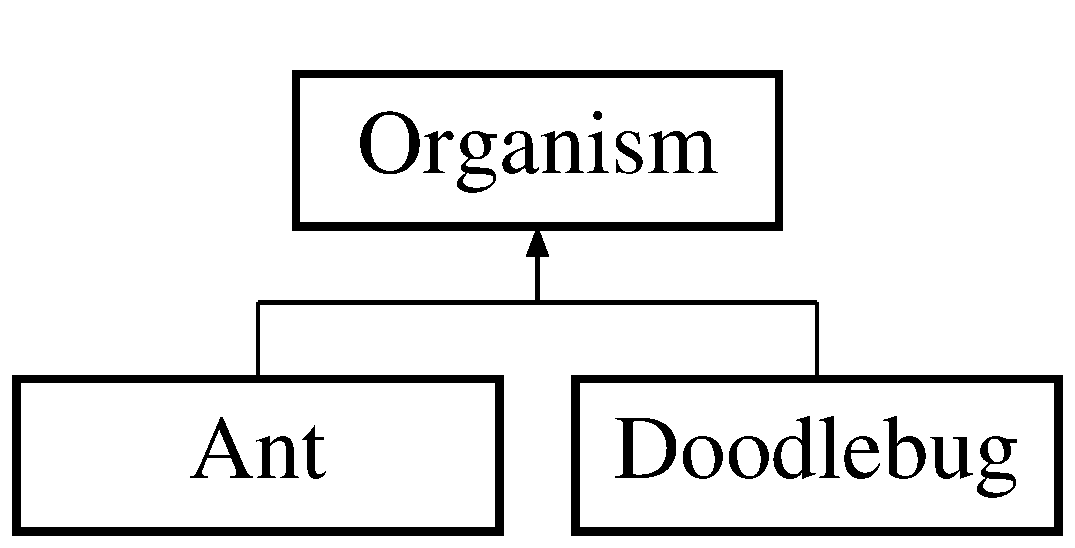
\includegraphics[height=2.000000cm]{classOrganism}
\end{center}
\end{figure}
\subsection*{Public Member Functions}
\begin{DoxyCompactItemize}
\item 
\textbf{ Organism} ()
\item 
\textbf{ Organism} (bool b)
\item 
bool \textbf{ is\+Prey} ()
\item 
virtual int \textbf{ move} (\textbf{ Grid} $\ast$grid)=0
\item 
virtual bool \textbf{ breed} (\textbf{ Grid} $\ast$grid)=0
\item 
void \textbf{ set\+Am\+Ant} (bool b)
\item 
virtual \textbf{ $\sim$\+Organism} ()
\end{DoxyCompactItemize}


\subsection{Constructor \& Destructor Documentation}
\mbox{\label{classOrganism_aeb16ee24b64839584b4862384d0b53fe}} 
\index{Organism@{Organism}!Organism@{Organism}}
\index{Organism@{Organism}!Organism@{Organism}}
\subsubsection{Organism()\hspace{0.1cm}{\footnotesize\ttfamily [1/2]}}
{\footnotesize\ttfamily Organism\+::\+Organism (\begin{DoxyParamCaption}{ }\end{DoxyParamCaption})}

\mbox{\label{classOrganism_ac7d3dbebaf5df39d0a7883b2d76b4868}} 
\index{Organism@{Organism}!Organism@{Organism}}
\index{Organism@{Organism}!Organism@{Organism}}
\subsubsection{Organism()\hspace{0.1cm}{\footnotesize\ttfamily [2/2]}}
{\footnotesize\ttfamily Organism\+::\+Organism (\begin{DoxyParamCaption}\item[{bool}]{b }\end{DoxyParamCaption})}



References am\+Ant.

\mbox{\label{classOrganism_aa5aa2e9fc3134358c929fa0c9d230c3b}} 
\index{Organism@{Organism}!````~Organism@{$\sim$\+Organism}}
\index{````~Organism@{$\sim$\+Organism}!Organism@{Organism}}
\subsubsection{$\sim$\+Organism()}
{\footnotesize\ttfamily Organism\+::$\sim$\+Organism (\begin{DoxyParamCaption}{ }\end{DoxyParamCaption})\hspace{0.3cm}{\ttfamily [virtual]}}



\subsection{Member Function Documentation}
\mbox{\label{classOrganism_a423246fb1dee94db6c8c3b08fba57ead}} 
\index{Organism@{Organism}!breed@{breed}}
\index{breed@{breed}!Organism@{Organism}}
\subsubsection{breed()}
{\footnotesize\ttfamily virtual bool Organism\+::breed (\begin{DoxyParamCaption}\item[{\textbf{ Grid} $\ast$}]{grid }\end{DoxyParamCaption})\hspace{0.3cm}{\ttfamily [pure virtual]}}



Implemented in \textbf{ Doodlebug} \doxyref{}{p.}{classDoodlebug_a6ab3919da6f9404f1f3af05f0bbde13c}, and \textbf{ Ant} \doxyref{}{p.}{classAnt_af899faded61186f5ca27e43cee1463ba}.

\mbox{\label{classOrganism_aa5213b2e2b0c4f227dc7dfc4c4ab411c}} 
\index{Organism@{Organism}!is\+Prey@{is\+Prey}}
\index{is\+Prey@{is\+Prey}!Organism@{Organism}}
\subsubsection{is\+Prey()}
{\footnotesize\ttfamily bool Organism\+::is\+Prey (\begin{DoxyParamCaption}{ }\end{DoxyParamCaption})}



References am\+Ant.

\mbox{\label{classOrganism_a2627a1917b919ab131d40d868b966020}} 
\index{Organism@{Organism}!move@{move}}
\index{move@{move}!Organism@{Organism}}
\subsubsection{move()}
{\footnotesize\ttfamily virtual int Organism\+::move (\begin{DoxyParamCaption}\item[{\textbf{ Grid} $\ast$}]{grid }\end{DoxyParamCaption})\hspace{0.3cm}{\ttfamily [pure virtual]}}



Implemented in \textbf{ Doodlebug} \doxyref{}{p.}{classDoodlebug_a5f28800e091fbeaabd57079b0c36e997}, and \textbf{ Ant} \doxyref{}{p.}{classAnt_a6806cb12fd6e7eea2ff74ea8aa33ce28}.



Referenced by Tests2\+::ants\+Breed\+Test(), Tests2\+::ants\+Die\+Test(), Tests2\+::ants\+Move\+Test(), Tests2\+::doodle\+Breed\+Test(), Tests2\+::doodle\+Dietest(), Tests2\+::doodle\+Move\+Test(), and Production\+::run\+Production().

\mbox{\label{classOrganism_aba68f4745f6b0938cf157dcd27df1868}} 
\index{Organism@{Organism}!set\+Am\+Ant@{set\+Am\+Ant}}
\index{set\+Am\+Ant@{set\+Am\+Ant}!Organism@{Organism}}
\subsubsection{set\+Am\+Ant()}
{\footnotesize\ttfamily void Organism\+::set\+Am\+Ant (\begin{DoxyParamCaption}\item[{bool}]{b }\end{DoxyParamCaption})}



References am\+Ant.



The documentation for this class was generated from the following files\+:\begin{DoxyCompactItemize}
\item 
\textbf{ Organism.\+h}\item 
\textbf{ Organism.\+cpp}\end{DoxyCompactItemize}

\section{Production Class Reference}
\label{classProduction}\index{Production@{Production}}


{\ttfamily \#include $<$Production.\+h$>$}

\subsection*{Public Member Functions}
\begin{DoxyCompactItemize}
\item 
\textbf{ Production} (int argc, char $\ast$argv[$\,$])
\item 
bool \textbf{ run\+Production} ()
\item 
virtual \textbf{ $\sim$\+Production} ()
\end{DoxyCompactItemize}
\subsection*{Data Fields}
\begin{DoxyCompactItemize}
\item 
int \textbf{ seed} =1
\item 
int \textbf{ timesteps\+Left} =1000
\item 
int \textbf{ grid\+Size} =20
\item 
int \textbf{ num\+Doodlebugs} =5
\item 
int \textbf{ num\+Ants} =100
\item 
int \textbf{ pause} =0
\end{DoxyCompactItemize}


\subsection{Constructor \& Destructor Documentation}
\mbox{\label{classProduction_a24439558b7672feaea80dc0ab1b53ff2}} 
\index{Production@{Production}!Production@{Production}}
\index{Production@{Production}!Production@{Production}}
\subsubsection{Production()}
{\footnotesize\ttfamily Production\+::\+Production (\begin{DoxyParamCaption}\item[{int}]{argc,  }\item[{char $\ast$}]{argv[$\,$] }\end{DoxyParamCaption})}



References arg\+Set\+Up, grid\+Size, num\+Ants, num\+Doodlebugs, pause, seed, and timesteps\+Left.



Referenced by main().

\mbox{\label{classProduction_ab5b3060f9e0a2bc189844e426d693dab}} 
\index{Production@{Production}!````~Production@{$\sim$\+Production}}
\index{````~Production@{$\sim$\+Production}!Production@{Production}}
\subsubsection{$\sim$\+Production()}
{\footnotesize\ttfamily Production\+::$\sim$\+Production (\begin{DoxyParamCaption}{ }\end{DoxyParamCaption})\hspace{0.3cm}{\ttfamily [virtual]}}



Referenced by main().



\subsection{Member Function Documentation}
\mbox{\label{classProduction_a1d66853eafae2580089eff44f12f07ba}} 
\index{Production@{Production}!run\+Production@{run\+Production}}
\index{run\+Production@{run\+Production}!Production@{Production}}
\subsubsection{run\+Production()}
{\footnotesize\ttfamily bool Production\+::run\+Production (\begin{DoxyParamCaption}{ }\end{DoxyParamCaption})}



References ant, arg\+Set\+Up, doodlebug, empty, Grid\+::get\+Board(), Grid\+::get\+Cell\+Occupant(), Cell\+::get\+Ptr(), grid\+Size, Organism\+::move(), Cell\+::\+New\+Ptr(), num\+Ants, num\+Doodlebugs, pause, Grid\+::print\+Grid(), Grid\+::rand\+Int(), seed, Grid\+::set\+Cell\+Occupant(), and timesteps\+Left.



Referenced by main().



\subsection{Field Documentation}
\mbox{\label{classProduction_aec26b656d2e7519d1a1898810bd1c0da}} 
\index{Production@{Production}!grid\+Size@{grid\+Size}}
\index{grid\+Size@{grid\+Size}!Production@{Production}}
\subsubsection{grid\+Size}
{\footnotesize\ttfamily int Production\+::grid\+Size =20}



Referenced by Production(), and run\+Production().

\mbox{\label{classProduction_a9bf1f5e66a3a787f08d37d5ef06cf8b6}} 
\index{Production@{Production}!num\+Ants@{num\+Ants}}
\index{num\+Ants@{num\+Ants}!Production@{Production}}
\subsubsection{num\+Ants}
{\footnotesize\ttfamily int Production\+::num\+Ants =100}



Referenced by Production(), and run\+Production().

\mbox{\label{classProduction_a3bfd9e01f9f73efd1f92176e5f7458eb}} 
\index{Production@{Production}!num\+Doodlebugs@{num\+Doodlebugs}}
\index{num\+Doodlebugs@{num\+Doodlebugs}!Production@{Production}}
\subsubsection{num\+Doodlebugs}
{\footnotesize\ttfamily int Production\+::num\+Doodlebugs =5}



Referenced by Production(), and run\+Production().

\mbox{\label{classProduction_af570feb7415a4d5b1a9176dacd9d6b64}} 
\index{Production@{Production}!pause@{pause}}
\index{pause@{pause}!Production@{Production}}
\subsubsection{pause}
{\footnotesize\ttfamily int Production\+::pause =0}



Referenced by Production(), and run\+Production().

\mbox{\label{classProduction_adb474287b0143fccb9d440ccc54ba624}} 
\index{Production@{Production}!seed@{seed}}
\index{seed@{seed}!Production@{Production}}
\subsubsection{seed}
{\footnotesize\ttfamily int Production\+::seed =1}



Referenced by main(), Production(), and run\+Production().

\mbox{\label{classProduction_a5fcf03b482712c458184ae4fd3f8e461}} 
\index{Production@{Production}!timesteps\+Left@{timesteps\+Left}}
\index{timesteps\+Left@{timesteps\+Left}!Production@{Production}}
\subsubsection{timesteps\+Left}
{\footnotesize\ttfamily int Production\+::timesteps\+Left =1000}



Referenced by Production(), and run\+Production().



The documentation for this class was generated from the following files\+:\begin{DoxyCompactItemize}
\item 
\textbf{ Production.\+h}\item 
\textbf{ Production.\+cpp}\end{DoxyCompactItemize}

\section{Tests2 Class Reference}
\label{classTests2}\index{Tests2@{Tests2}}


{\ttfamily \#include $<$Tests2.\+h$>$}

\subsection*{Public Member Functions}
\begin{DoxyCompactItemize}
\item 
\textbf{ Tests2} ()
\item 
bool \textbf{ do\+Tests} ()
\item 
bool \textbf{ grid\+Test} ()
\item 
bool \textbf{ make\+Ants\+Test} ()
\item 
bool \textbf{ ants\+Move\+Test} ()
\item 
bool \textbf{ ants\+Move\+Test1} ()
\item 
bool \textbf{ ants\+Breed\+Test} ()
\item 
bool \textbf{ ants\+Die\+Test} ()
\item 
bool \textbf{ make\+Doodles\+Test} ()
\item 
bool \textbf{ doodle\+Move\+Test} ()
\item 
bool \textbf{ doodle\+Move\+Test1} ()
\item 
bool \textbf{ doodle\+Breed\+Test} ()
\item 
bool \textbf{ doodle\+Eat\+Test} ()
\item 
bool \textbf{ doodle\+Dietest} ()
\item 
virtual \textbf{ $\sim$\+Tests2} ()
\end{DoxyCompactItemize}


\subsection{Constructor \& Destructor Documentation}
\mbox{\label{classTests2_a6d7d8d248dd3d544199769baa1face60}} 
\index{Tests2@{Tests2}!Tests2@{Tests2}}
\index{Tests2@{Tests2}!Tests2@{Tests2}}
\subsubsection{Tests2()}
{\footnotesize\ttfamily Tests2\+::\+Tests2 (\begin{DoxyParamCaption}{ }\end{DoxyParamCaption})}

\mbox{\label{classTests2_abed1a850ef511b7c06ae418cb3bbd5d9}} 
\index{Tests2@{Tests2}!````~Tests2@{$\sim$\+Tests2}}
\index{````~Tests2@{$\sim$\+Tests2}!Tests2@{Tests2}}
\subsubsection{$\sim$\+Tests2()}
{\footnotesize\ttfamily Tests2\+::$\sim$\+Tests2 (\begin{DoxyParamCaption}{ }\end{DoxyParamCaption})\hspace{0.3cm}{\ttfamily [virtual]}}



Referenced by main().



\subsection{Member Function Documentation}
\mbox{\label{classTests2_a21e7692afbdfb694caf370670cbeb7d4}} 
\index{Tests2@{Tests2}!ants\+Breed\+Test@{ants\+Breed\+Test}}
\index{ants\+Breed\+Test@{ants\+Breed\+Test}!Tests2@{Tests2}}
\subsubsection{ants\+Breed\+Test()}
{\footnotesize\ttfamily bool Tests2\+::ants\+Breed\+Test (\begin{DoxyParamCaption}{ }\end{DoxyParamCaption})}



References ant, Grid\+::get\+Board(), Cell\+::get\+Ptr(), Organism\+::move(), Cell\+::\+New\+Ptr(), and Grid\+::set\+Cell\+Occupant().



Referenced by do\+Tests().

\mbox{\label{classTests2_a045d58417814d72bcf4c97b2ebb51461}} 
\index{Tests2@{Tests2}!ants\+Die\+Test@{ants\+Die\+Test}}
\index{ants\+Die\+Test@{ants\+Die\+Test}!Tests2@{Tests2}}
\subsubsection{ants\+Die\+Test()}
{\footnotesize\ttfamily bool Tests2\+::ants\+Die\+Test (\begin{DoxyParamCaption}{ }\end{DoxyParamCaption})}



References ant, doodlebug, Grid\+::get\+Board(), Cell\+::get\+Ptr(), Organism\+::move(), Cell\+::\+New\+Ptr(), Grid\+::print\+Grid(), and Grid\+::set\+Cell\+Occupant().



Referenced by do\+Tests().

\mbox{\label{classTests2_a7694d2797eba6fadc40234d527f6afbe}} 
\index{Tests2@{Tests2}!ants\+Move\+Test@{ants\+Move\+Test}}
\index{ants\+Move\+Test@{ants\+Move\+Test}!Tests2@{Tests2}}
\subsubsection{ants\+Move\+Test()}
{\footnotesize\ttfamily bool Tests2\+::ants\+Move\+Test (\begin{DoxyParamCaption}{ }\end{DoxyParamCaption})}



References ant, Grid\+::get\+Board(), Cell\+::get\+Ptr(), Organism\+::move(), Cell\+::\+New\+Ptr(), and Grid\+::set\+Cell\+Occupant().



Referenced by do\+Tests().

\mbox{\label{classTests2_ad3b43320ed586fe37b8feba46ddbd0bd}} 
\index{Tests2@{Tests2}!ants\+Move\+Test1@{ants\+Move\+Test1}}
\index{ants\+Move\+Test1@{ants\+Move\+Test1}!Tests2@{Tests2}}
\subsubsection{ants\+Move\+Test1()}
{\footnotesize\ttfamily bool Tests2\+::ants\+Move\+Test1 (\begin{DoxyParamCaption}{ }\end{DoxyParamCaption})}

\mbox{\label{classTests2_a317dc926bf93038f188c999df7a85682}} 
\index{Tests2@{Tests2}!doodle\+Breed\+Test@{doodle\+Breed\+Test}}
\index{doodle\+Breed\+Test@{doodle\+Breed\+Test}!Tests2@{Tests2}}
\subsubsection{doodle\+Breed\+Test()}
{\footnotesize\ttfamily bool Tests2\+::doodle\+Breed\+Test (\begin{DoxyParamCaption}{ }\end{DoxyParamCaption})}



References ant, doodlebug, Grid\+::get\+Board(), Cell\+::get\+Ptr(), Organism\+::move(), Cell\+::\+New\+Ptr(), Grid\+::print\+Grid(), and Grid\+::set\+Cell\+Occupant().



Referenced by do\+Tests().

\mbox{\label{classTests2_aaf403f9bb7338771173e2053ea4f95fc}} 
\index{Tests2@{Tests2}!doodle\+Dietest@{doodle\+Dietest}}
\index{doodle\+Dietest@{doodle\+Dietest}!Tests2@{Tests2}}
\subsubsection{doodle\+Dietest()}
{\footnotesize\ttfamily bool Tests2\+::doodle\+Dietest (\begin{DoxyParamCaption}{ }\end{DoxyParamCaption})}



References doodlebug, Grid\+::get\+Board(), Cell\+::get\+Ptr(), Organism\+::move(), Cell\+::\+New\+Ptr(), Grid\+::print\+Grid(), and Grid\+::set\+Cell\+Occupant().



Referenced by do\+Tests().

\mbox{\label{classTests2_ae35f30e7d95e581cc4ce1316409c71ac}} 
\index{Tests2@{Tests2}!doodle\+Eat\+Test@{doodle\+Eat\+Test}}
\index{doodle\+Eat\+Test@{doodle\+Eat\+Test}!Tests2@{Tests2}}
\subsubsection{doodle\+Eat\+Test()}
{\footnotesize\ttfamily bool Tests2\+::doodle\+Eat\+Test (\begin{DoxyParamCaption}{ }\end{DoxyParamCaption})}



Referenced by do\+Tests().

\mbox{\label{classTests2_a2143f2192836626e7214d37b504df381}} 
\index{Tests2@{Tests2}!doodle\+Move\+Test@{doodle\+Move\+Test}}
\index{doodle\+Move\+Test@{doodle\+Move\+Test}!Tests2@{Tests2}}
\subsubsection{doodle\+Move\+Test()}
{\footnotesize\ttfamily bool Tests2\+::doodle\+Move\+Test (\begin{DoxyParamCaption}{ }\end{DoxyParamCaption})}



References doodlebug, Grid\+::get\+Board(), Cell\+::get\+Ptr(), Organism\+::move(), Cell\+::\+New\+Ptr(), and Grid\+::set\+Cell\+Occupant().



Referenced by do\+Tests().

\mbox{\label{classTests2_a836becfa6b79d5f2113940a11a3ef47e}} 
\index{Tests2@{Tests2}!doodle\+Move\+Test1@{doodle\+Move\+Test1}}
\index{doodle\+Move\+Test1@{doodle\+Move\+Test1}!Tests2@{Tests2}}
\subsubsection{doodle\+Move\+Test1()}
{\footnotesize\ttfamily bool Tests2\+::doodle\+Move\+Test1 (\begin{DoxyParamCaption}{ }\end{DoxyParamCaption})}

\mbox{\label{classTests2_a7392382310966597d685c8aa3a4a2f88}} 
\index{Tests2@{Tests2}!do\+Tests@{do\+Tests}}
\index{do\+Tests@{do\+Tests}!Tests2@{Tests2}}
\subsubsection{do\+Tests()}
{\footnotesize\ttfamily bool Tests2\+::do\+Tests (\begin{DoxyParamCaption}{ }\end{DoxyParamCaption})}



References ants\+Breed\+Test(), ants\+Die\+Test(), ants\+Move\+Test(), doodle\+Breed\+Test(), doodle\+Dietest(), doodle\+Eat\+Test(), doodle\+Move\+Test(), grid\+Test(), make\+Ants\+Test(), and make\+Doodles\+Test().



Referenced by main().

\mbox{\label{classTests2_afe90de3a79c4105e63205cb8f019bbb2}} 
\index{Tests2@{Tests2}!grid\+Test@{grid\+Test}}
\index{grid\+Test@{grid\+Test}!Tests2@{Tests2}}
\subsubsection{grid\+Test()}
{\footnotesize\ttfamily bool Tests2\+::grid\+Test (\begin{DoxyParamCaption}{ }\end{DoxyParamCaption})}



References ant, empty, Grid\+::get\+Cell\+Occupant(), Grid\+::set\+Cell\+Occupant(), and Grid\+::$\sim$\+Grid().



Referenced by do\+Tests().

\mbox{\label{classTests2_aa4d40396194cf770aa82dc11b449ea62}} 
\index{Tests2@{Tests2}!make\+Ants\+Test@{make\+Ants\+Test}}
\index{make\+Ants\+Test@{make\+Ants\+Test}!Tests2@{Tests2}}
\subsubsection{make\+Ants\+Test()}
{\footnotesize\ttfamily bool Tests2\+::make\+Ants\+Test (\begin{DoxyParamCaption}{ }\end{DoxyParamCaption})}



References ant, doodlebug, empty, Grid\+::get\+Cell\+Occupant(), and Grid\+::set\+Cell\+Occupant().



Referenced by do\+Tests().

\mbox{\label{classTests2_a0c6c7e5d60e7c6dc8799fa14e2b997b4}} 
\index{Tests2@{Tests2}!make\+Doodles\+Test@{make\+Doodles\+Test}}
\index{make\+Doodles\+Test@{make\+Doodles\+Test}!Tests2@{Tests2}}
\subsubsection{make\+Doodles\+Test()}
{\footnotesize\ttfamily bool Tests2\+::make\+Doodles\+Test (\begin{DoxyParamCaption}{ }\end{DoxyParamCaption})}



Referenced by do\+Tests().



The documentation for this class was generated from the following files\+:\begin{DoxyCompactItemize}
\item 
\textbf{ Tests2.\+h}\item 
\textbf{ Tests2.\+cpp}\end{DoxyCompactItemize}

\chapter{File Documentation}
\section{Ant.\+cpp File Reference}
\label{Ant_8cpp}\index{Ant.\+cpp@{Ant.\+cpp}}
{\ttfamily \#include \char`\"{}Ant.\+h\char`\"{}}\newline
{\ttfamily \#include \char`\"{}Grid.\+h\char`\"{}}\newline
{\ttfamily \#include \char`\"{}Cell.\+h\char`\"{}}\newline

\section{Ant.\+h File Reference}
\label{Ant_8h}\index{Ant.\+h@{Ant.\+h}}
{\ttfamily \#include \char`\"{}Organism.\+h\char`\"{}}\newline
{\ttfamily \#include \char`\"{}Grid.\+h\char`\"{}}\newline
\subsection*{Data Structures}
\begin{DoxyCompactItemize}
\item 
class \textbf{ Ant}
\end{DoxyCompactItemize}

\section{Ants\+And\+Doodles.\+cpp File Reference}
\label{AntsAndDoodles_8cpp}\index{Ants\+And\+Doodles.\+cpp@{Ants\+And\+Doodles.\+cpp}}
{\ttfamily \#include $<$iostream$>$}\newline
{\ttfamily \#include $<$stdlib.\+h$>$}\newline
{\ttfamily \#include \char`\"{}Tests2.\+h\char`\"{}}\newline
{\ttfamily \#include \char`\"{}Production.\+h\char`\"{}}\newline
\subsection*{Functions}
\begin{DoxyCompactItemize}
\item 
int \textbf{ main} (int argc, char $\ast$argv[$\,$])
\end{DoxyCompactItemize}


\subsection{Function Documentation}
\mbox{\label{AntsAndDoodles_8cpp_a0ddf1224851353fc92bfbff6f499fa97}} 
\index{Ants\+And\+Doodles.\+cpp@{Ants\+And\+Doodles.\+cpp}!main@{main}}
\index{main@{main}!Ants\+And\+Doodles.\+cpp@{Ants\+And\+Doodles.\+cpp}}
\subsubsection{main()}
{\footnotesize\ttfamily int main (\begin{DoxyParamCaption}\item[{int}]{argc,  }\item[{char $\ast$}]{argv[$\,$] }\end{DoxyParamCaption})}



References Tests2\+::do\+Tests(), Production\+::\+Production(), Production\+::run\+Production(), Production\+::seed, Production\+::$\sim$\+Production(), and Tests2\+::$\sim$\+Tests2().


\section{Cell.\+cpp File Reference}
\label{Cell_8cpp}\index{Cell.\+cpp@{Cell.\+cpp}}
{\ttfamily \#include \char`\"{}Cell.\+h\char`\"{}}\newline
{\ttfamily \#include \char`\"{}Organism.\+h\char`\"{}}\newline
{\ttfamily \#include \char`\"{}Ant.\+h\char`\"{}}\newline
{\ttfamily \#include \char`\"{}Doodlebug.\+h\char`\"{}}\newline

\section{Cell.\+h File Reference}
\label{Cell_8h}\index{Cell.\+h@{Cell.\+h}}
\subsection*{Data Structures}
\begin{DoxyCompactItemize}
\item 
class \textbf{ Cell}
\end{DoxyCompactItemize}
\subsection*{Enumerations}
\begin{DoxyCompactItemize}
\item 
enum \textbf{ occupation\+Status} \{ \textbf{ empty}, 
\textbf{ ant}, 
\textbf{ doodlebug}
 \}
\end{DoxyCompactItemize}


\subsection{Enumeration Type Documentation}
\mbox{\label{Cell_8h_abcce8bf608a2504bf718b7234aa15acb}} 
\index{Cell.\+h@{Cell.\+h}!occupation\+Status@{occupation\+Status}}
\index{occupation\+Status@{occupation\+Status}!Cell.\+h@{Cell.\+h}}
\subsubsection{occupation\+Status}
{\footnotesize\ttfamily enum \textbf{ occupation\+Status}}

\begin{DoxyEnumFields}{Enumerator}
\raisebox{\heightof{T}}[0pt][0pt]{\index{empty@{empty}!Cell.\+h@{Cell.\+h}}\index{Cell.\+h@{Cell.\+h}!empty@{empty}}}\mbox{\label{Cell_8h_abcce8bf608a2504bf718b7234aa15acbae8654263bd8adf1d0922f427d8f3fc1b}} 
empty&\\
\hline

\raisebox{\heightof{T}}[0pt][0pt]{\index{ant@{ant}!Cell.\+h@{Cell.\+h}}\index{Cell.\+h@{Cell.\+h}!ant@{ant}}}\mbox{\label{Cell_8h_abcce8bf608a2504bf718b7234aa15acbacc8f2f9c5b15a05a2f336152b3794aa9}} 
ant&\\
\hline

\raisebox{\heightof{T}}[0pt][0pt]{\index{doodlebug@{doodlebug}!Cell.\+h@{Cell.\+h}}\index{Cell.\+h@{Cell.\+h}!doodlebug@{doodlebug}}}\mbox{\label{Cell_8h_abcce8bf608a2504bf718b7234aa15acba55f311222a925986c2589e11b469c0f2}} 
doodlebug&\\
\hline

\end{DoxyEnumFields}

\section{Doodlebug.\+cpp File Reference}
\label{Doodlebug_8cpp}\index{Doodlebug.\+cpp@{Doodlebug.\+cpp}}
{\ttfamily \#include \char`\"{}Doodlebug.\+h\char`\"{}}\newline
{\ttfamily \#include \char`\"{}Grid.\+h\char`\"{}}\newline

\section{Doodlebug.\+h File Reference}
\label{Doodlebug_8h}\index{Doodlebug.\+h@{Doodlebug.\+h}}
{\ttfamily \#include \char`\"{}Organism.\+h\char`\"{}}\newline
{\ttfamily \#include \char`\"{}Grid.\+h\char`\"{}}\newline
\subsection*{Data Structures}
\begin{DoxyCompactItemize}
\item 
class \textbf{ Doodlebug}
\end{DoxyCompactItemize}

\section{Grid.\+cpp File Reference}
\label{Grid_8cpp}\index{Grid.\+cpp@{Grid.\+cpp}}
{\ttfamily \#include $<$iostream$>$}\newline
{\ttfamily \#include $<$iomanip$>$}\newline
{\ttfamily \#include \char`\"{}Grid.\+h\char`\"{}}\newline
{\ttfamily \#include \char`\"{}Cell.\+h\char`\"{}}\newline

\section{Grid.\+h File Reference}
\label{Grid_8h}\index{Grid.\+h@{Grid.\+h}}
{\ttfamily \#include \char`\"{}Cell.\+h\char`\"{}}\newline
\subsection*{Data Structures}
\begin{DoxyCompactItemize}
\item 
class \textbf{ Grid}
\end{DoxyCompactItemize}

\section{Organism.\+cpp File Reference}
\label{Organism_8cpp}\index{Organism.\+cpp@{Organism.\+cpp}}
{\ttfamily \#include \char`\"{}Organism.\+h\char`\"{}}\newline
{\ttfamily \#include \char`\"{}Grid.\+h\char`\"{}}\newline
\subsection*{Variables}
\begin{DoxyCompactItemize}
\item 
bool \textbf{ am\+Ant} = false
\end{DoxyCompactItemize}


\subsection{Variable Documentation}
\mbox{\label{Organism_8cpp_a900bc6f8ceeedef124e764e3c72b1735}} 
\index{Organism.\+cpp@{Organism.\+cpp}!am\+Ant@{am\+Ant}}
\index{am\+Ant@{am\+Ant}!Organism.\+cpp@{Organism.\+cpp}}
\subsubsection{am\+Ant}
{\footnotesize\ttfamily bool am\+Ant = false}



Referenced by Organism\+::is\+Prey(), Organism\+::\+Organism(), and Organism\+::set\+Am\+Ant().


\section{Organism.\+h File Reference}
\label{Organism_8h}\index{Organism.\+h@{Organism.\+h}}
{\ttfamily \#include \char`\"{}Grid.\+h\char`\"{}}\newline
\subsection*{Data Structures}
\begin{DoxyCompactItemize}
\item 
class \textbf{ Organism}
\end{DoxyCompactItemize}

\section{Production.\+cpp File Reference}
\label{Production_8cpp}\index{Production.\+cpp@{Production.\+cpp}}
{\ttfamily \#include \char`\"{}Production.\+h\char`\"{}}\newline
{\ttfamily \#include $<$stdlib.\+h$>$}\newline
{\ttfamily \#include $<$iostream$>$}\newline
{\ttfamily \#include \char`\"{}Grid.\+h\char`\"{}}\newline
{\ttfamily \#include \char`\"{}Organism.\+h\char`\"{}}\newline
\subsection*{Variables}
\begin{DoxyCompactItemize}
\item 
bool \textbf{ arg\+Set\+Up} =true
\item 
\textbf{ Grid} $\ast$ \textbf{ final\+Grid}
\end{DoxyCompactItemize}


\subsection{Variable Documentation}
\mbox{\label{Production_8cpp_a93df441d853a9c6e32f2725da66fa38b}} 
\index{Production.\+cpp@{Production.\+cpp}!arg\+Set\+Up@{arg\+Set\+Up}}
\index{arg\+Set\+Up@{arg\+Set\+Up}!Production.\+cpp@{Production.\+cpp}}
\subsubsection{arg\+Set\+Up}
{\footnotesize\ttfamily bool arg\+Set\+Up =true}



Referenced by Production\+::\+Production(), and Production\+::run\+Production().

\mbox{\label{Production_8cpp_acea9cff1e9553dfffe9a5769e0eb6d27}} 
\index{Production.\+cpp@{Production.\+cpp}!final\+Grid@{final\+Grid}}
\index{final\+Grid@{final\+Grid}!Production.\+cpp@{Production.\+cpp}}
\subsubsection{final\+Grid}
{\footnotesize\ttfamily \textbf{ Grid}$\ast$ final\+Grid}


\section{Production.\+h File Reference}
\label{Production_8h}\index{Production.\+h@{Production.\+h}}
\subsection*{Data Structures}
\begin{DoxyCompactItemize}
\item 
class \textbf{ Production}
\end{DoxyCompactItemize}

\section{Tests2.\+cpp File Reference}
\label{Tests2_8cpp}\index{Tests2.\+cpp@{Tests2.\+cpp}}
{\ttfamily \#include \char`\"{}Tests2.\+h\char`\"{}}\newline
{\ttfamily \#include \char`\"{}Grid.\+h\char`\"{}}\newline
{\ttfamily \#include \char`\"{}Ant.\+h\char`\"{}}\newline
{\ttfamily \#include \char`\"{}Doodlebug.\+h\char`\"{}}\newline
{\ttfamily \#include $<$iostream$>$}\newline
{\ttfamily \#include \char`\"{}Cell.\+h\char`\"{}}\newline

\section{Tests2.\+h File Reference}
\label{Tests2_8h}\index{Tests2.\+h@{Tests2.\+h}}
\subsection*{Data Structures}
\begin{DoxyCompactItemize}
\item 
class \textbf{ Tests2}
\end{DoxyCompactItemize}

%--- End generated contents ---

% Index
\backmatter
\newpage
\phantomsection
\clearemptydoublepage
\addcontentsline{toc}{chapter}{Index}
\printindex

\end{document}
